\chapter{The Level 3 / Data Acquisition System}
\label{Level3} 

\section{Introduction}

The Data Acquisition System and Level3 Trigger at Fermilab's \dzero\
Experiment assembles data from 63 VME crates each containing
1-20kB/event spread through 1-10 VME modules into complete 250kB
events in one of 82 farm nodes at a 1kHz event rate. The events are
run through fast reconstruction and 50Hz is selected and sent to
tape storage. Up to 8 simultaneous runs are supported, allowing for
flexible data taking, commissioning, and calibration. Near-real-time
monitoring of each component is provided to many graphical displays
of various types. Commodity hardware such as the CISCO 6509 Ethernet
switch, open-source software such as ACE [2] and Linux, and the
standard TCP/IP protocol are used throughout. The system has
performed well since commissioning in July, 2002.

\section{Hardware Components}

\begin{figure}
\centering
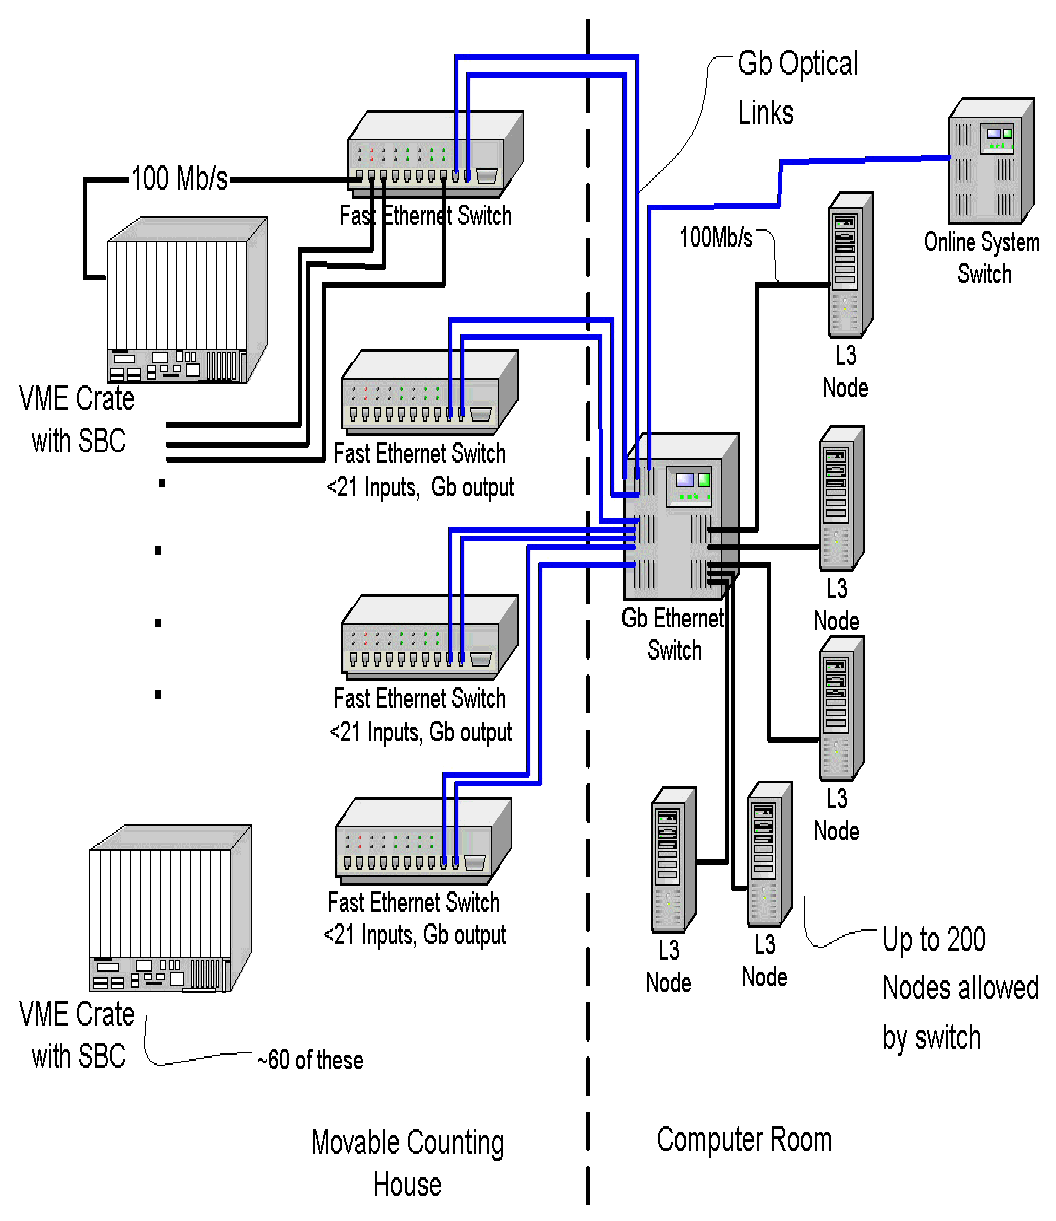
\includegraphics[width=6in,height=6in]{eps/Level3/L3-DAQ.eps}
\caption{Hardware components.} \label{DAQ_Hardware}
\end{figure}

The system is composed of Single-board Computers (SBCs), 100~Mb/s to
Gb/s Ethernet converter switches (CISCO 2948Gs), a single main
Ethernet switch (CISCO 6509), and computer farm nodes. The
components and their connections are shown in
Figure~\ref{DAQ_Hardware}. The SBCs send data from their VME crates
over dual 100~Mb/s Ethernet connections to the 2948Gs which transfer
the data to the main switch over Gb/s optical fibers. The farm nodes
are connected to the main switch by 100~Mb/s Ethernet connections.

\subsection{Single-Board Computers}

The SBCs have two jobs in the system: they are readout controllers
for the event data, and one hosts the Routing Master program which
coordinates the others. The VMIC 7750~\cite{VMIC} SBC being used has
a 933~MHz Pentium-III processor, 128~MB of RAM, 128~MB of flash ROM
(used for booting), fast VME access, one PMC expansion slot, and two
100~Mb/s Ethernet interfaces. The VMIC SBCs use the Tundra Universe
II ~\cite{Tundra} chip for the VME-PCI interface. The Universe II is
compliant with 32 or 64-bit VME transfers, has a programmable DMA
controller, offers flexible interrupt logic, and allows address
pipelining, which is used in reading out some of the VME crates. The
single PMC slot is occupied by a BVM~\cite{BVM} digital I/O module,
used for coordinating the readout of VME modules over the VME J3
connector. Additional PMC slots can be added through an additional
VME card, which may be used in the future to expand the Ethernet
capabilities using Gb/s adapters.

The sole custom hardware component in the system is the extender
board used to mechanically support the 6U commercial SBCs in the 9U
readout crates, propagate signals to the panel at the front of the
VME crate, and connect lines on the digital I/O card to the J3
backplane.

\subsection{Ethernet Switches}

Two types of Ethernet switches are used. A set of CISCO 2948G's act
as concentrators, transferring packets from up to ten 100~Mb/s
connections to Gb/s optical fibers. The number of 100~Mb/s
connections is limited to ensure no network congestion occurs at
this stage. The Gb fiber links are brought together in a central
switch (the CISCO 6509) to which the farm nodes are also connected.
The central switch can handle an effective bandwidth of 16~GB/s,
which is more than sufficient for the peak dataflow of 500~MB/s. The
CISCO 6509 can be configured with up to 9 modules. One module is
being used to provide the 100~Mb/s Ethernet ports (for the farm
nodes). This module also has 112~MB of output buffer memory shared
between the 48 ports. Another module contains the Gb/s optical fiber
inputs (for accepting data from the 2948Gs).

\subsection{Farm Nodes}

Programs on the farm nodes build events from the data fragments
received, reconstruct the events, and perform physics selection. The
computers used are dual 1~GHz Pentium III rack-mounted machines with
1 GB of RAM, two 100~Mb/s Ethernet ports, and a small amount of
local disk. There are currently 82 nodes, but the system is
expandable to handle more than two times as many (limited only by
the number of modules that can be added to the central switch).

\section{Software Components}

\begin{figure}
\centering
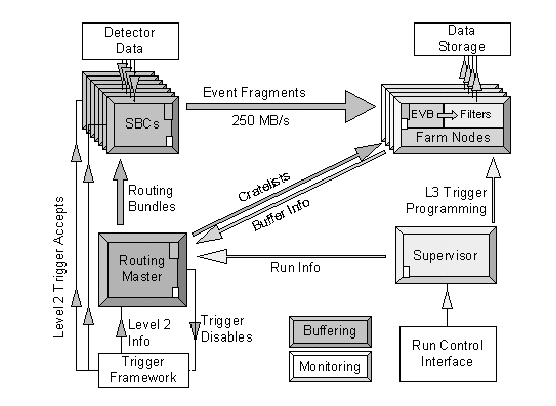
\includegraphics[width=5in]{eps/Level3/daq_software.eps}
\caption{Software components, showing dataflow and feedback.}
\label{DAQ Software}
\end{figure}

Custom software performs the logic used for reading out the VME
crates, buffering and routing the event data, sending and receiving
data across the Ethernet network, assembling the event fragments
into complete events, and deciding whether the event should be kept
or discarded.

Three main types of information need to be transmitted (and
received): crate data, routing information, and node free-buffer
information. In addition, monitoring information, remote commands,
and configuration information also need to be passed, although at a
lower rate and at lower priority. The TCP Ethernet protocol is used
to transmit this data through the network with negligible loss or
corruption, at high rate, with low latency, while consuming a
minimum of CPU power cycles to send and receive. Although the UDP
protocol was considered for broadcasting routing commands to the
SBCs, TCP was chosen in the end for its predicable performance under
heavy network load.

Instead of directly implementing our own TCP socket calls, the
ACE~\cite{ACE} C++ Network Framework is used, which wraps this
functionality while adding a negligible performance overhead. In
addition, the ACE library offers many useful patterns such as thread
management, thread-safe queues, timers, and de-multiplexing event
handlers, through a platform independent, object-oriented interface.
In particular, the \emph{Task} construct, which combines an input
and output queue with a worker thread, is the building block of all
the routing and communication software.

\subsection{Supervisor}

The D\O\ experiment's data taking is controlled by shifters, who
interact with run control software (COOR). The DAQ is designed to
handle multiple simultaneous definitions of L1/L2/L3 triggers, each
loosely referred to as a \emph{run}. The Supervisor program provides
the interface between COOR and the DAQ/L3 system. When a new run is
configured, the Supervisor receives configuration information which
specifies the node resources to allocate to this run, the type of
code to have the nodes execute, the VME crates that will be read out
for each event in this run, and the trigger configuration, which
contains a description of the requirements events have to satisfy to
pass the L3 trigger. The Supervisor initializes the appropriate
nodes and tells the Routing Master about this new run. The run can
then be started and paused an unlimited number of times, and the
Supervisor communicates the new state to the Routing Master so that
it can decide whether to allow events to be sent to nodes in the
run. When the run is stopped, the Supervisor instructs the nodes to
return to their un-configured state, and downloads new programming
to the Routing Master which no longer includes information about
this run.

If an error occurs while the Supervisor is trying to change the
state of the system, the change is aborted, and the whole system is
restored to the last valid state. The error message is returned to
the run-control system so that proper recovery steps can be taken.
Programs which unexpectedly crash or are intentionally stopped and
restarted are automatically reconfigured without shifter
intervention.

\subsection{Routing Master}

The Routing Master program executes on an SBC in a special crate
whose data contains information about which L1/L2 triggers passed.
The RM's job is to synchronize and direct the sending of data from
all the other read-out crates to one or more farm nodes for each
event. The crate housing the RM also has special hardware
connections back to the trigger framework, which the Routing Master
can use to disable L1 triggers, to apply back-pressure when the L2
accept rate is too high.

The Supervisor configures the Routing Master with a set of runs that
share farm resources through a strict set of rules. A run is a set
of available nodes and triggers and a set of required crates that
must be read out for each trigger. After each L2 trigger accept, the
Routing Master reads data out of the special trigger crate and, for
each run which overlaps with at least one of the passed L1/L2
triggers, it chooses one node to be used for the event. This
decision of which node to choose for each run is based on the number
of available event \emph{buffers} in each node. The Routing Master
maintains an internal table of free buffers for each node, called
the Node Free-buffer Map. Each time an event is routed to a node the
corresponding entry in the Node Free-buffer Map is decremented by
one. The entries are incremented periodically when the RM receives
messages from the nodes, which indicate a number of event buffers
that the node has freed. A node is chosen in a round-robin fashion
from amongst the set of nodes with the most free buffers, to divide
events amongst equally free nodes most evenly.

If too few free node buffers in a run are available (as determined
from the Node Free-buffer Map), the Routing Master communicates over
VME to other specialized cards in the crate it is housed to apply
back-pressure to the L1 trigger system by disabling the triggers
associated with that run. The triggers are re-enabled when a node in
the run informs the Routing Master that free buffers are available
again. The algorithm employed guarantees that the SBCs will not be
instructed to send data to a node until the node is able to
internally buffer the event immediately.

A set of VME crates to be read out for each run is generated by
making the union of all the trigger lists associated with the L1/L2
triggers that passed for the event. The Routing Master creates a
route command for each SBC which is in a VME crate in this set of
crates. The route command is an integer representing the event
number and a set of node indices indicating the nodes to which the
SBC should send the data for this event. When all runs have been
considered for an event, the route commands are added to routing
bundles, which group together route commands for multiple events
into a single message. This grouping is necessary to reduce the
number of TCP messages sent out over Ethernet by the Routing Master,
since there is a per-message overhead. A routing bundle containing a
non-zero number of routing commands is sent out either after 250~ms
or when it contains some maximum number (by default 10) of routing
commands. A bundle is also sent early occasionally (.1\% of events)
to add randomization, such that not all routing bundles are sent
after the same event.

The Routing Master also sends information to each chosen node for
each event: the event number, the crate list, and the fired L1/L2
triggers. The event number and crate list are required for the node
to know when it has received data from all the crates needed for the
event. The trigger list is needed for reporting to monitoring about
which triggers were associated with an event, especially if the
event was incomplete due to an error. Properly counting the number
of events recorded for each trigger is crucial (for calculating the
luminosity accurately).

In summary, the Routing Master polls a VME location connected to the
Trigger Framework every 10ms and reads a list of Event Tags,
containing a 16 bit L3 event number and a list of passed L2 trigger
bits. For each Event Tag, it builds the list of runs which have at
least one of its L2 trigger bits in the Event Tag. For each of these
runs in the list:
\begin{itemize}
  \item A Farm Node is chosen from the list of Farm Nodes in the run,
  based on which has the most free buffers in the Node Free-Buffer Map.
  \item For each L2 trigger bit in the Event Tag, the list of crates to
   be read out for that L2 trigger bit is added to the set of crates to be read out.
  \item The chosen Farm Node is sent a Cratelist containing the L3 event number,
   the L2 trigger bit list in the Event Tag, and the set of crates that will be read out.
  \item The index of the chosen Farm Node is added to a Route Tag to be sent to
  each crate in the set of crates to be read out. Each Route Tag is added the
  Routing Bundle for its SBC, which is soon sent to the SBC.
  \item If less than 16 Farm Node buffers are available, the trigger bits for
  the run are disabled. They are re-enabled when 24 Farm Node buffers in the run are free.
\end{itemize}

\subsection{Read-Out Processes}

The software running on the SBC in each standard read-out crate must
read out the data from other modules in the crate and send it to the
nodes, as instructed by routing commands from the Routing Master.
The Linux operating system is used on the SBCs for conformity with
the majority of other systems in the experiment and to take
advantage of local expertise. Two main processes run on each board:
\begin{itemize}
\item
The Interrupt Service Routine (ISR) is a kernel module which waits
on a custom kernel interrupt initiated by a request for read-out
communicated through the J3 VME connector to the BVM DIO module in
the SBC's PMC slot. The ISR starts the data transfer (carried out
through DMA) into a buffer in the SBC's memory. The buffers are
created in kernel-space memory at boot-time through a specialized
kernel module. The buffers are used in circular order, and two
pointers keep track of the first and last buffer used, such that the
data is never copied. This design, in particular the choice of
putting functionality directly into the kernel itself, minimizes
latency by avoiding the Linux scheduler.
\item
The Event Sender is a user-level process that receives routing
information from the Routing Master and attempts to match it (by
event number) with event data in buffers pointed to by the ISR. If
the event number in a route command matches the event number in a
data buffer, the Event Sender transmits the buffer's data to the
specified node(s). If the event numbers do not match, a warning is
issued, either the event data or the route command is discarded
(based on which event number was behind), and a new match is
attempted. This way, the Event Sender keeps itself synchronized even
when routing or event data is occasionally missing or duplicated.
\end{itemize}

\subsection{Farm Nodes}

Three main types of processes execute on each farm node, also under
the Linux operating system. These processes are managed by a Program
Manager on each node, which can start the correct version of
software, restart crashed processes, and stop processes.
\begin{itemize}
\item
The Event Builder (EVB) combines event fragments, received from SBCs
in the VME crates, into complete events. Event fragments are
organized into complete events through the use of a map, keyed by
event number. Data is read over Ethernet from the SBCs and buffered
in a fixed-length input queue. Another thread processes event
fragments in the input queue and places pointers to the fragments
into the map. A map entry is marked as complete when it contains
pointers to fragments from all the SBCs required, as specified by
the crate-list sent to it by the Routing Master for that event. The
fragments are then copied (concatenated) into a contiguous memory
buffer provided by \emph{IO Process} (see below) and deleted from
the map. Map entries which are still incomplete after one second are
erased, and the associated fragments are deleted. Incomplete events
are carefully reported to the \emph{Monitor Server} (see below).
Whenever a map entry is freed, a message is sent to the Routing
Master to inform it that space for another event is available,
unless too many free buffers are already being advertised to the RM
(see \emph{Buffering} below).
\item
The IO Process takes complete events that have been built by the EVB
and distributes them between the multiple L3 Filter processes (see
below). Two L3 filter processes are needed to take advantage of both
CPU's on each farm node.
\item
The L3 Filter processes reconstruct each physics event and decide if
it passed or failed the programmed filter requirements. A passed
event is sent over 100~Mb/s Ethernet to a dedicated machine called
the Collector, and failed events are discarded.
\end{itemize}

\subsection{Monitor Server}

The ability to retrieve detailed information from all software
components in the system in near-real time (within a few tens of
milliseconds) is crucial for debugging, troubleshooting, and
understanding the performance of the system. The Monitor Server is
software which runs on a dedicated commodity PC (similar to those
used for receiving events), and coordinates the efficient gathering
of this information.

All software components in the system (a total of over a hundred)
connect to the Monitor Server as \emph{clients}, and are able to
respond to it with extensive statistics and other information about
their status. The Monitor Server responds to queries from
\emph{displays}, such as a web-page scripts and graphical programs.
The display's query can request any set of information from any set
of components in the system. The Monitor Server then makes queries
of the necessary client components, collects the information
asynchronously as it is returned from the clients, and sends back a
response containing the information initially requested by the
display. The type of information gathered is very diverse, from
event rates to the status of TCP connections to idle CPU time.

XML is used for all communications with the Monitor Server, as
opposed to unstructured binary or textual data. The format is
flexible enough to handle any kind of information transfer, safe and
fast to parse in almost any language on almost any platform, and
humanly readable for debugging purposes. The XERCES~\cite{XERCES}
parser was chosen for use in all C++ components for its speed, wide
acceptance and support in the community, and ability to run on a
wide variety of platforms.

The Monitor Server must be able to support a large number of
displays operating worldwide, making simultaneous queries. However,
there is some overhead in gathering information from a client, so
care must be taken not to query clients too frequently, or the
data-taking performance of the system would be degraded. Therefore,
the Monitor Server caches information that it has gathered, so that
no client will be bothered to report the same information more than
once per second, no matter how frequently the server is queried.

\section{Buffering}

\begin{figure}
\centering
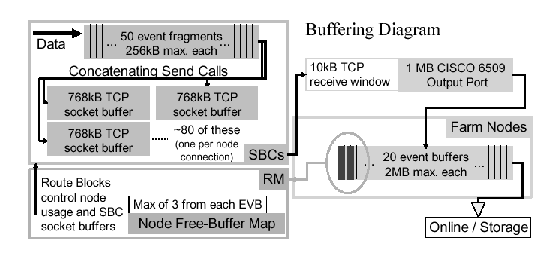
\includegraphics[width=5in]{eps/Level3/buffering.eps}
\caption{Buffering controls.} \label{Buffering}
\end{figure}

Operation of the DAQ at high rates requires that buffers be
available to absorb latencies in the system or there will be
unacceptable dead-time. In general, buffering exists almost
everywhere data or other messages are transferred over Ethernet
between machines and between threads or processes on the same
machine.

Buffering in the system is adequate to sustain continuous data flow
at full rate. The Routing Master controls data flow, based on
free-buffer information fed back from the Farm Nodes, to take
advantage of the distributed buffering throughout the system. If
back-up occurs in or downstream of the Farm Nodes, the lack of
advertised free-buffers from the Farm Nodes causes the Routing
Master to disable triggers via the Trigger Framework interface
before buffers in the system overflow.

Data read out over VME by an SBC is placed into one of 50 statically
allocated, fixed-size kernel-memory buffers. These buffers are used
in a circular order, with head and tail pointers indicating the
first and last used buffer, respectively.

Queues that can each hold approximately 100 routing commands exist
in the RM to buffer the routing bundles waiting to be sent to each
connected SBC. A corresponding queue in each SBC Event Sender
program, of the same maximum size, buffers the routing messages on
the receiving end as they are waiting to be matched with
corresponding data read out from their VME crates.

Data sent from the SBCs to the farm nodes is buffered by the
kernel-level TCP socket buffers. The connection's \emph{send-buffer}
size is set to 768~kB on the SBC, which provides about 100 event
data fragment buffers on average (comparable to the routing message
buffer). On the farm node, a queue with a maximum size of 40
fragments buffers event data fragments being received from all the
SBCs. Fragments are buffered here until they are copied into the
EVB's input queue, which has a maximum length of 700 fragments
(enough to hold about 10 events). The EVB's event map can hold the
pieces of at most 20 events at a time. IO Process then buffers these
events until they are processed by one of the L3 filter processes.
Finally, those events which pass the L3 trigger requirements are
passed to a final output queue, where they wait to be sent to the
Collector, a central machine that gathers events to be written to
tape for offline analysis.

The number of event buffers the farm nodes \emph{advertise} to the
Routing Master (3) is not the full number they have available (20).
The farm nodes each report a much smaller number of free buffers to
ensure that the RM does not send out routing to an SBC that would
cause it to fill up its TCP output socket buffer (causing the SBC to
hang because it uses a blocking TCP send call). Since the maximum
event fragment size is 256~kB, and the socket buffer size is 768~kB,
the node only advertises 3 buffers at any one time to the RM. This
is acceptable because, in total, the 82 farm nodes thus advertises
246 event buffers, more than in the SBCs.

The messages sent from the farm nodes to the Routing Master are
buffered in a queue on each node which can hold a maximum of 100
messages. Once received in the RM, the messages are processed
immediately by the receiving thread to make the free node buffer
usable again as soon as possible.

In summary, the following buffers and controls are used:
\begin{itemize}
\item Each SBC has 50 event fragment buffers in Linux kernel memory, where event
fragments wait to be concatenated into TCP socket buffers.
\item There is a large 768kB TCP socket buffer on each SBC $\rightarrow$ Farm Node connection.
They can not fill up and block, since the maximum crate size is
256kB and the Routing Master only routes a maximum of 3 events to a
Farm Node at a time. Ensuring that send calls will not block
simplifies the event sending logic.
\item The TCP\_RTO\_MIN compile-time Linux TCP parameter was changed from the 200ms
default to 10ms in the Routing Master to assure no delays in Routing
Bundle delivery due to occasional packet loss.
\item Each output port on the CISCO 6509 has a 1MB buffer. The Farm Node TCP
receive window size is kept at 10kB per SBC connection to not
overflow the switch's output port buffer. (~80 SBC connections x
10kB/connection $<$ 1MB)
\item The EVB has 20 event buffers where event fragments are built into complete
events. Only 3 are advertised to the Routing Master, to not overflow
the SBCs' TCP socket buffers.
\item Events are held in 3 shared memory buffers waiting for the Filters to
process them.
\end{itemize}

\section{Control}

\subsection{Software Versioning and Distribution}

An efficient and easily usable set of scripts exists for controlling
the software that runs on each of the machines in the system. The
currently active version of software on each machine can be
specified from a central location. A version of software can be
automatically distributed to machines if it does not already exist
locally. The \emph{rgang}~\cite{RGANG} command is used to distribute
the software efficiently, as well as to execute remote commands on
multiple machines simultaneously.

\subsection{Initialization}

When programs involved with data-flow start up, they read a single
cross-mounted (using NFS) XML file which defines the \emph{topology}
of the system. The file describes the DNS names of all the SBCs and
farm nodes, assigns each node a unique index, and maps each SBC to
its unique crate-id. These indices and crate-id's are used to
identify each process in communicated messages at runtime. The
topology file also identifies the location of the Supervisor,
Routing Master, SBCs, and Monitor Server. Using this information,
appropriate TCP connections are established between components in
the system. The SBCs and farm nodes make the connection to the RM,
since the RM's address is stable whereas addresses of other
components, or even the number of them, can change over time. The
farm nodes connect to the SBC's so that if a farm node crashes, it
can reconnect to the SBC's when it is restarted.

\subsection{Runtime Control}

The Supervisor does the majority of the runtime control of the
system, however it is often useful to be able to \emph{manually}
change the parameters of some set of processes while they are
running, particularly while debugging or testing. To accomplish
this, a configuration port is opened on the Routing Master and each
SBC. A special command-line program (executed either locally or
remotely) can connect to this port and alter some parameters. For
instance, in the Routing Master, the maximum number of routing
commands in a routing group can be modified. In the SBCs, the
compression settings (see below) can be changed, and an additional
\emph{stream} or file can be created for collecting some or all
events. This last feature has been very useful for detector groups
as they debug their systems.

\section{Stability and Robustness}

Several features were designed into the system to increase its
stability and robustness, even in the face of unexpected mechanical,
computational, or (most importantly) human errors. Every connection
ensures that it is still viable by sending intermittent \emph{pings}
(either a short string or an empty TCP packet). If any connection is
determined to be closed, either from the failure of a ping, or from
the detection of a closed TCP socket, the remote machine is polled
at a 10 second interval until the connection is re-established.

Most connections are also protected against hangs in the case that
data can not be sent or received for some reason. There are 15
second timeouts on the sending or receiving of messages in many
places, in case a remote machine is not behaving as expected. When
receiving, checks are made that there is room to store the new data,
and if there isn't, a warning is issued, and the oldest information
is overwritten. (This can not occur unless a failure somewhere else
in the system has caused the buffering logic to fail.) When sending,
separate threads are often used to prevent an entire process from
being blocked by one hung connection.

Many \emph{sanity checks} are also included. For instance, the Event
Builder periodically (at least every 5 seconds) re-communicates its
availability to the Routing Master, in order to guarantee
synchronization.

Also, the system is designed such that any set of machines or
processes (with the exception of the Supervisor) can be restarted
without adversely affecting the rest of the system. Often, runs can
continue unaffected, if they are not directly using the component
being restarted, such as when a node or an SBC is restarted. If the
Routing Master is restarted, all runs will stop until the needed
components have reconnected to it, at which time all runs will
resume automatically, without external intervention.

\section{Ethernet Bandwidth Optimization}

While the total bandwidth of the system is easily handled by the
main CISCO 6509 switch, the maximum rate of the whole system is
limited by the slowest crate. The bottleneck will most likely be the
Ethernet transfer of data from a crate to nodes. Thus, care has been
taken to optimize the Ethernet bandwidth out of the crates.

\subsection{Dual Ethernet Interface Utilization}

Each SBC has two 100~Mb/s Ethernet ports, and thus a maximum
theoretical output bandwidth of about 24~MB/s. (Additional daughter
cards can be added to the SBCs to give them GB/s Ethernet output.)
Pooling the output bandwidth of both interfaces (which are on the
same sub-net) to send data to a set of nodes is non-trivial,
however. An Ethernet packet being routed by the operating system to
any two nodes on the same sub-net will by default always choose the
same hardware interface to use (unless explicit entries are added to
the routing table for each node), regardless of which interface the
connection was established on.

This default routing behavior can be avoided by using the
BINDTODEVICE~\cite{SO_BINDTODEVICE} socket option under Linux.
Sockets are opened on two different ports, and each is bound to a
separate hardware interface. Each node then makes a connection to
each socket. The SBC alternates between the two ports on consecutive
sends to different nodes and also on consecutive events to
distribute the data most evenly between the interfaces.

\subsection{Dynamic Compression}

Additional effective bandwidth can be achieved by compressing the
data before it is sent, using a lossless compression algorithm, and
then uncompressing it in the node. Two compression algorithms are
available, and can be selected dynamically (see \emph{runtime
control} above). The gzip~\cite{zlib} algorithm offers the best
compression factor, but uses a lot of CPU to compress the data. The
lzo\_1x~\cite{lzo} algorithm is amongst the fastest of compression
algorithms, but does not achieve as great a compression ratio. To
prevent the SBC from becoming CPU-limited, the fraction of events
which are subjected to compression is dynamically adjusted to use
less than 100\% of the CPU power. In addition, in order not to waste
CPU time, the fraction of compressed events is adjusted dynamically
so that if the output bandwidth falls below a certain limit, the
amount of compression is reduced.

\section{Offline Testing}

Since all components must be continuously operational, software
changes need to be tested \emph{offline} as much as possible, before
being applied to the real system. The Routing Master, Event Sender,
and Event Builder can be run in a \emph{test} mode, which fully
tests their code and simulates any inputs or hardware which do not
exist. The Routing Master, for instance, can simulate incoming
triggers at any desired rate. A full test, containing all these
components, can be run on a single machine or multiple machines, and
has been automated by simple scripts. In addition, the tests can be
run under the Linux or Win32 platforms (or a combination), which
helps to find odd bugs or race conditions that behave differently
under the subtleties of each platform.

A test-crate which houses an SBC is used for testing new read-out
hardware or software configurations. The data for the test crate can
come from a variety of sources.

\section{System Performance}

The system has been running online continuously for over a year, and
many tests have been performed. The performance of the full system
has surpassed its design expectations.

The bandwidth output of the dual 100~Mb/s Ethernet interfaces of an
SBC has been shown in the test crate to sustain greater than 22~MB/s
sending to 4 nodes, each of which has a single 100~Mb/s Ethernet
interface. The CPU consumption on the SBC was around 20\%. Using the
lzo\_1x compression, average event data could be sent at over
30~MB/s, using nearly all of the SBC's CPU power.

High-rate tests have been run with up to 6 SBCs and 24 nodes. The
Routing Master consumed about 30\% CPU at 2~kHz. The CPU usage did
not increase appreciably as more SBCs or nodes were added to the
test (since the real work is in making the routing decisions
themselves).

The Event Builder uses less than 10\% of a CPU to build full events
from 60 crates at 100~Hz. Recall that at the design rate of the
system (1~kHz), each node only needs to process events at 20~Hz.

Downloading a new run is the most time-consuming control operation,
since a large amount of information must be distributed to and
parsed by each node. By sending commands in parallel, the Supervisor
is able to program a farm of 24 nodes and the Routing Master in
about 5 seconds total.

During normal running, there are routinely more than 50 monitor
displays running in the control room and throughout the world. The
Monitor Server typically has about 150 total clients connected, from
which data is available. Gathering 10~kB of XML from a client takes
about 10~ms. Responding to a query which demands gathering 300~kB of
XML in total from all 90 clients takes about 50~ms, since
information is gathered in parallel. The Monitor Server uses about
20\% of its CPU power while serving about 500~kB/s of XML spread
amongst many displays.

\section{Conclusions}

The software components rely upon high level programming languages;
the Linux operating system; widely�-used, open libraries; and
standard networking protocols. The routing and buffering methods
have performed reliably since commissioning and satisfy the current
and future needs of the \dzero\ experiment.

Using commercial hardware (SBCs, Ethernet switches, PC farm nodes)
and widely-used software libraries (ACE, XERCES, etc.) helped to
significantly reduce the amount of time necessary to design and
implement a full Data Acquisition system. The SBCs are more than
sufficient for simultaneously reading out data in the VME crates,
receiving routing information, and sending the data over Ethernet to
the chosen farm nodes. The Routing Master is able to generate and
send routing messages to all the SBCs at beyond the required rate.
The buffering strategies, monitoring system, software version
control, and runtime control also work well. In addition to playing
a critical role in our current experiment, this system is expandable
to fulfill future DAQ needs at D\O\ and elsewhere.
